%----------------------------------------------------------------------------------------
%	PACKAGES AND OTHER DOCUMENT CONFIGURATIONS
%----------------------------------------------------------------------------------------

\documentclass[twoside]{article}

\usepackage[sc]{mathpazo} % Use the Palatino font
\usepackage[T1]{fontenc} % Use 8-bit encoding that has 256 glyphs
\linespread{1.05} % Line spacing - Palatino needs more space between lines
\usepackage{microtype} % Slightly tweak font spacing for aesthetics

\usepackage[english]{babel} % Language hyphenation and typographical rules

\usepackage[hmarginratio=1:1,top=32mm,columnsep=20pt]{geometry} % Document margins
\usepackage[hang, small,labelfont=bf,up,textfont=it,up]{caption} % Custom captions under/above floats in tables or figures
\usepackage{booktabs} % Horizontal rules in tables

\usepackage{lettrine} % The lettrine is the first enlarged letter at the beginning of the text

\usepackage{enumitem} % Customized lists
\setlist[itemize]{noitemsep} % Make itemize lists more compact

\usepackage{titlesec} % Allows customization of titles
\renewcommand\thesection{\Roman{section}} % Roman numerals for the sections
\renewcommand\thesubsection{\roman{subsection}} % roman numerals for subsections
\titleformat{\section}[block]{\large\scshape\centering}{\thesection.}{1em}{} % Change the look of the section titles
\titleformat{\subsection}[block]{\large}{\thesubsection.}{1em}{} % Change the look of the section titles

\usepackage{fancyhdr} % Headers and footers
\pagestyle{fancy} % All pages have headers and footers
\fancyhead{} % Blank out the default header
\fancyfoot{} % Blank out the default footer
\fancyhead[C]{Search for Exoplanets $\bullet$ April 2018} % Custom header text
\fancyfoot[RO,LE]{\thepage} % Custom footer text

\usepackage{titling} % Customizing the title section

\usepackage{hyperref} % For hyperlinks in the PDF

\usepackage{multicol}
\usepackage{graphicx}
\graphicspath{{img/}}
\usepackage{float}
\usepackage{cite}

\newcommand{\code}[1]{\texttt{#1}}

%----------------------------------------------------------------------------------------
%	TITLE SECTION
%----------------------------------------------------------------------------------------

\setlength{\droptitle}{-4\baselineskip} % Move the title up

\pretitle{\begin{center}\Huge\bfseries} % Article title formatting
\posttitle{\end{center}} % Article title closing formatting
\title{Search for Exoplanets\\ \large \textit{\\(project proposal)}} % Article title

\author{%
\textsc{Petra Br\v{c}i\'c}\\%\thanks{The greatest mathematician} \\[1ex] 
\normalsize Applied Mathematics \\
\normalsize \href{mailto:petrabrcic94@gmail.com}{petrabrcic94@gmail.com} 
\and
\textsc{Sandro Lovni\v{c}ki}\\%\thanks{The greatest logician} \\[1ex] 
\normalsize Computer Science \\ 
\normalsize \href{mailto:lovnicki.sandro@gmail.com}{lovnicki.sandro@gmail.com}
}

\date{\today} 
\renewcommand{\maketitlehookd}{%
\noindent \textbf{\\Abstract:}
With the launch of Kepler space observatory in March 2009, the search for exoplanets has extensively began. There are currently $3,758$ confirmed exoplanets and contrary to the early approaches of validating exoplanet candidates by hand, machine learning has begun taking its toll on the subject. We would like to investigate neural network model for detecting transiting exoplanets from Kepler observatory light-curve data collected over a period of $4$ years, with over $200,000$ documented stars in our galaxy, the Milky Way. On April 18, 2018, a new satellite (TESS) has been launched, specificaly designed to search for exoplanets using the transit method. After it's 2-year planned mission, complete data should be available to public and more than $20,000$ new exoplanets are expected to be found.
\\\\
\textbf{Keywords:} Kepler, light-curve, exoplanet, machine learning, neural network, TESS.
}


%----------------------------------------------------------------------------------------

\begin{document}

% Print the title and table of contents
\maketitle
%\tableofcontents
%\newpage

%----------------------------------------------------------------------------------------
%	ARTICLE CONTENTS
%----------------------------------------------------------------------------------------
\begin{multicols}{2}

\section{Introduction}
In March 2009, NASA launched Kepler space observatory to discover Earth-size planets orbiting other stars in our galaxy. With most of the discoveries made after Kepler data was anounced, there are currently $3,758$ confirmed exoplanets in $2,808$ systems, with $627$ systems having more than one planet. Contrary to the early approaches of validating exoplanet candidates by hand or with humanly constructed models, recent years have been fruitfull for usage of machine learning for classifing Kepler's data.

\section{Methods}
There are many methods for detecting an exoplanet existance, as it can be seen in \cite{exo:methods}.\\
For example, \textit{gravitational lensing} method exploits the stars' gravitational fields' effect on magnification of distant background stars' light. If the star in question has a planet, its gravitational field makes a detectable contribution to the lensing effect. Over the past 10 years, just a $1000$ such events have been observed because specific alignment of bodies is required. Nonetheless, 19 exoplanets have been discovered using this method, whose full list is given in \cite{microlensing:exos}.\\
It is notable to mention \textit{radial velocity} method which uses variations in the speed with which specific star moves away or towards the Earth. Those variations are influenced by orbiting planet's gravitational pull and therefore we can also deduce the planet's mass. Up to 2012, this method was most effective for exoplanet detection whose full list is given in \cite{radial:exos}.

The most effective method today is the \textit{transit photometry}. When a planet crosses (transits) in front of its star, the star's brightness diminishes depending on planet relative size to it. To detect those brightness variations, observer's relative position must be properly aligned with star-planet axis which is not something one can control. The probability of a random alignment producing a transit in a system with Sun-sized star and a planet at 1AU \footnote{1 Astronomical unit $\approx$ Earth's ditstance to the Sun $\approx$ 150 million kilometres} from it is $0.47\%$. Ilustration of how those brightness variations are manifested in Kepler's data can be seen in Figure \ref{fig:kepler_curves}.
\begin{figure}[H]
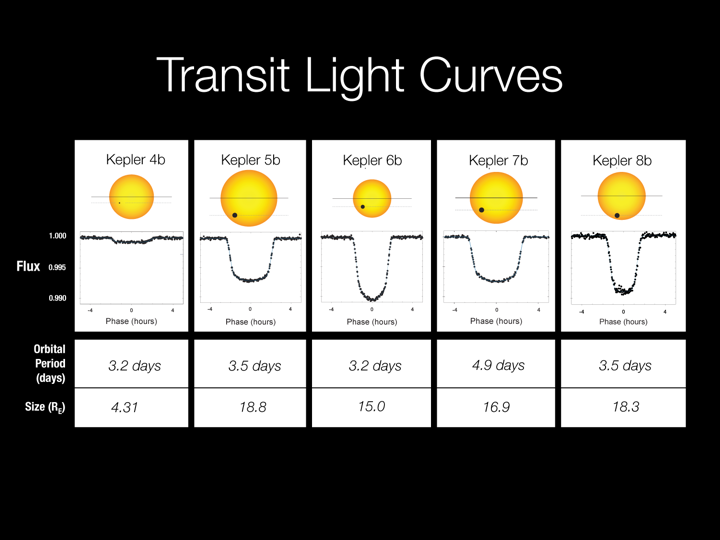
\includegraphics[width=0.5\textwidth]{KeplerLightCurves}
\caption{Illustration from \href{https://www.nasa.gov/mission_pages/kepler/main/index.html?FuseAction=ShowNews&NewsID=16}{Bill Borucki's Jan 2010 AAS Presentation}}
\label{fig:kepler_curves}
\end{figure}
\noindent Another disadvantage of this method is a high rate of false positives due to measurement precission and external noise that can be interpreted as a transit. For this reason, transit photometry is often combined with radial velocity to produce better results and eliminate false positives. The main advantage of transit photometry is planet's size deduction from light curve drops, which combined with transit photometry's mass deduction yields planet's density - a property much appriciated in search of habitable worlds. Also, by observing spectrum of light passed through the planet's atmosphere, one can detect which chemical elements are present. By April 12, 2018, Kepler detected $2,343$ exoplanets using transit photometry as a base method.



%------------------------------------------------

\section{Our approach}
In this section, we would like to loosely define our approach to the problem, base methods we will use and conclusions we would like to obtain.

\subsection{Models}
Based on previous section, transit photometry stems as the go-to method having in mind the Kepler mission and recent launch of TESS.
The amount of data will grow rapidly when TESS begins its mission, becoming unbearable for human examination. On the other hand, In the world of Machines, neural networks are getting their deserved popularity back and keep getting better and better at learning and predicting things (in comparison to their rival methods like Linear Regression, ...). Also, neural nets have given great results in detecting exoplanets from Kepler's light-curves as reported by \cite{Shallue:2017}. Correspondingly, we shall use appropriate programming tools and methods, all of which Python modules for scientific computing provide.

\subsection{Datasets}
Not all star's light-curves monitored by Kepler have a transit, but those transits that are periodic are called \textit{Threshold Crossing Events} (TCEs) which are then associated with their period, duration, etc. There are $20,367$ TCEs documented at \href{https://exoplanetarchive.ipac.caltech.edu/cgi-bin/TblView/nph-tblView?app=ExoTbls&config=q1_q17_dr24_tce}{NASA exoplanet archive} which have been processed and labeled by human scientists. From their labels, it can be deduced wheather a TCE is an orbiting planet or not, as well as many other useful features. We will use this dataset as our guidance to ensure our algorithms are working properly.\\
Next, for our raw training dataset, we will use Kepler's light-curves corresponding to stars in above dataset (have the same \code{kepid}). This can be found at \href{https://archive.stsci.edu/}{Mikulski archive for space telescopes}. Example of one plotted raw light-curve data can be seen in Figure \ref{fig:k90lc}
\begin{figure}[H]
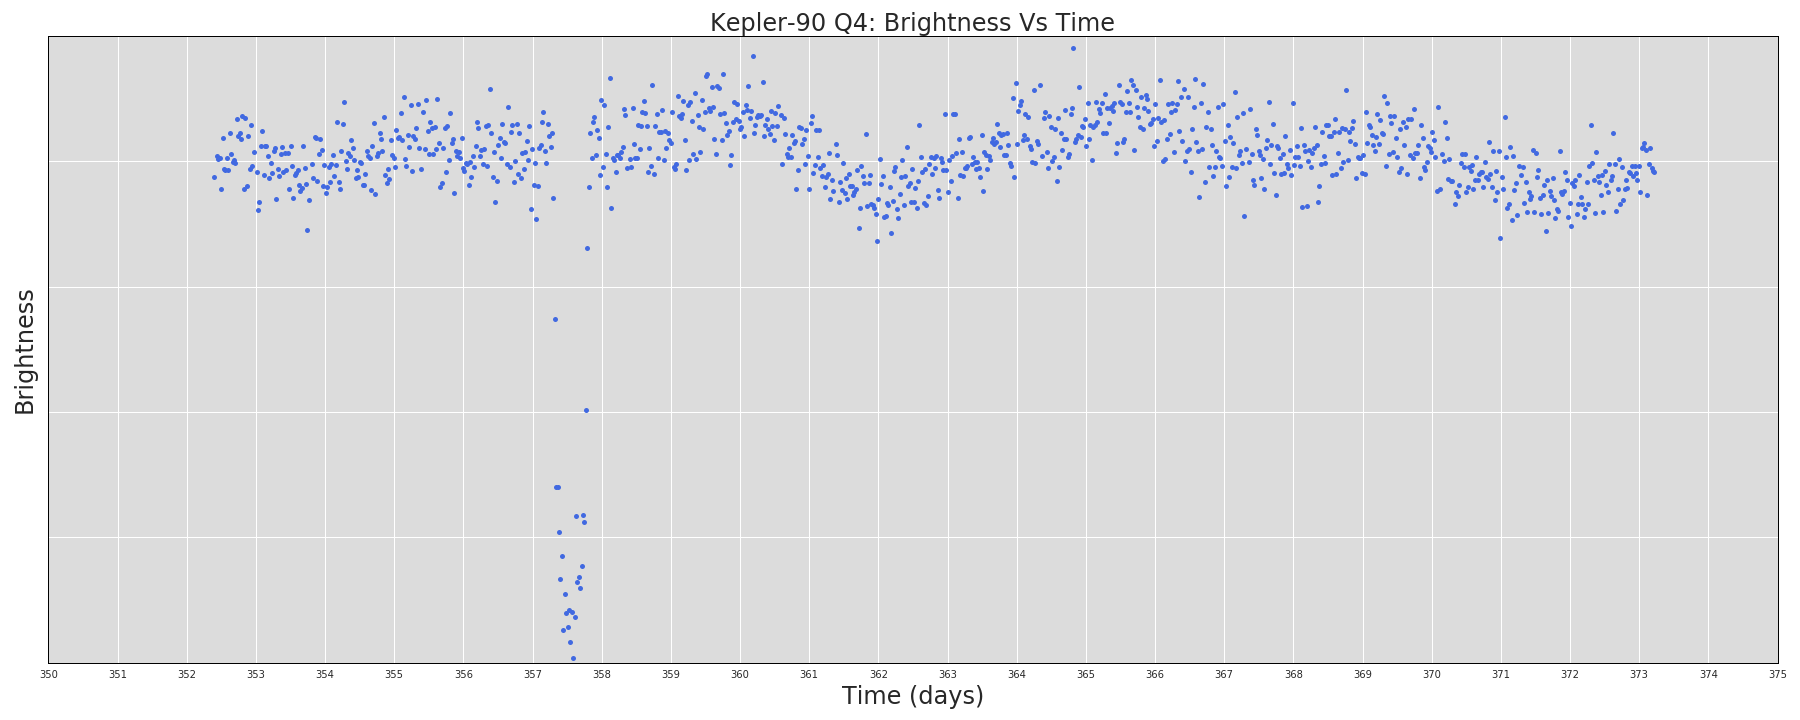
\includegraphics[width=0.5\textwidth]{kep90-q4-raw}
\caption{Light curve of Kepler-90 star}
\label{fig:k90lc}
\end{figure}

\subsection{Interpretations}
As we could have seen in Figure \ref{fig:k90lc}, objects of interest are drops in star's brightness, which, if are periodic and similar, could mean a planet is passing around the star with one revolution every period. Also, with some additional calculations, drop's depth represents the size of the planet. The hardest parth will be the distinction of false-positives, which could be from, e.g. eclipsing binaries \footnote{Systems that have two stars, orbiting eachother}, that are hard to distinguish visualy (\textit{Note: they could be distinguished by radial velocity method more easily}).\\
First, we expect our research to at least classify two groups of ligh-curves; those that have an TCE and thse that don't. It would be very desirable to be able to cut off most of the false positives. Finding a new exoplanet seems too improbable at the moment, but we are sure that project will continue its path for many years to prepare for TESS, therefore eventually finding at least one new exoplanet.


%------------------------------------------------

\section{Results and future}
As a result of our investigation of Kepler's data, we would like to end up with descent exoplanet detection algorithm using the transit method.
On April 18 this year, a new space satellite TESS (Transiting Exoplanet Survey Satellite) has been launched to specificly collect and process data for exoplanet search. It is expected to bring much more detailed data than Kepler, with many new useful features for each observed star. We will be able to detect not just an exoplanet's existance more easily, but also its atmosphere composition which should lead to discoveries of new habitable planets in our galactic neighbourhood.\\
We are eager to join the search.


%----------------------------------------------------------------------------------------
%	REFERENCE LIST
%----------------------------------------------------------------------------------------

\begin{thebibliography}{99}

\bibitem[1]{kepler:wiki}
\url{https://en.wikipedia.org/wiki/Kepler_(spacecraft)}

\bibitem[2]{tess:wiki}
\url{https://en.wikipedia.org/wiki/Transiting_Exoplanet_Survey_Satellite}

\bibitem[TESS]{tess}
\url{https://tess.mit.edu/}

\bibitem[3]{exo:methods}
\url{https://en.wikipedia.org/wiki/Methods_of_detecting_exoplanets}

\bibitem[4]{microlensing:exos}
\url{https://en.wikipedia.org/wiki/List_of_exoplanets_detected_by_microlensing}

\bibitem[5]{radial:exos}
\url{https://en.wikipedia.org/wiki/List_of_exoplanets_detected_by_radial_velocity}

\bibitem[6]{kepler:exos}
\url{https://en.wikipedia.org/wiki/List_of_exoplanets_discovered_using_the_Kepler_spacecraft}

\bibitem[Shallue and Vanderburg, 2017]{Shallue:2017}
Christopher J. Shallue, Andrew Vanderburg (2017).
\newblock Identifying Exoplanets with Deep Learning: A Five Planet Resonant Chain around Kepler-80 and an Eighth Planet around Kepler-90
\newblock arXiv:1712.05044 [astro-ph.EP]

\bibitem[Mikulski Archive for Space Telescopes]{mikulski}
\url{https://archive.stsci.edu/}

\bibitem[NASA Exoplanet Archive]{NASA:exos}
\url{https://exoplanetarchive.ipac.caltech.edu/cgi-bin/TblView/nph-tblView?app=ExoTbls&config=q1_q17_dr24_tce}

\bibitem[TCEs table]{tces}
\url{https://exoplanetarchive.ipac.caltech.edu/cgi-bin/TblView/nph-tblView?app=ExoTbls&config=q1_q17_dr24_tce}
 
\end{thebibliography}

%----------------------------------------------------------------------------------------

\end{multicols}{2}
\end{document}
